% ============================================================================
\section{Data Regimes and Structural Disjointness}
\label{sec:data}

\subsection{Corpus and repetition}
The corpus contains 1,595 anonymized enterprise IT tickets from one support
organization, each with a title, a description, the recorded resolving team
(37 teams), a reply-derived intent class (17 classes), and the historical first
reply that serves as the reference resolution. The source export contained 1,597
rows; two duplicate ticket references were removed. Every artifact in this paper
uses the same 1,595 canonical identifiers, so counts are comparable across the
earlier and revised analyses.

Repetition is substantial, and its form matters. The earlier cleaning pass
described 88 identical-reply groups covering 922 tickets. That statement conflated
two different relations. On the canonical corpus, 922 tickets share the first 300
characters of the normalized reply, while 238 share an identical normalized full
reply. The prefix relation is the conservative one: two tickets can open with the
same form or greeting and still describe different procedures. We therefore treat
the full-reply and prefix relations separately and never describe the 922 tickets
as identical replies.

\subsection{Structural groups}
We define two versioned rules over normalized signatures. The \emph{duplicate}
rule links two tickets when they have an identical normalized full reply or an
identical normalized title and subcategory. The \emph{prefix} rule additionally
links tickets whose replies share the first 300 normalized characters, using both
the earlier raw-cut definition and a normalized-cut definition. Groups are the
connected components of the resulting graph; an empty signature never links
tickets. The duplicate rule yields 1,218 components (largest 83); the prefix rule
yields 676 components (largest 299).

These rules are structural proxies, not semantic proof that two tickets follow the
same procedure. Two different procedures can share a template opening, and two
tickets with different wording can require the same action. We therefore call the
resulting panels \emph{structurally} disjoint and treat procedure identity as a
proxy, to be validated by the expert assessment in Section~\ref{sec:expert}. The
important property is that the proxy is defined without looking at any outcome and
is applied atomically to whole groups.

\subsection{Group-aware splits}
Whole groups are assigned to train, dev or eval, so no group crosses a partition
boundary. The duplicate split has 878/319/398 tickets; the prefix split has
856/312/427. The prefix split cannot hit 878/319/398 without cutting the
299-ticket component, which we refused to do. Five seeds were generated for each
rule; the primary analyses use seed 42 and the other seeds are reported as
robustness. No outcome enters the assignment.

The strict panel is the primary control because it removes both full-reply and
300-character-prefix overlap with training. The duplicate panel is the intermediate
control: it removes full-reply and title+subcategory duplicates but still allows a
shared reply opening. The familiar panel is the random split used in the earlier
evaluation. Table~\ref{tab:overlap} reports what each split actually guaranteed.

\Table[!btp](width=\textwidth){Evaluation tickets whose training partition contains
a ticket with the same structural signature. ``Duplicate union'' is the
connected-component rule over identical full reply or identical title+subcategory.
Counts are tickets; percentages are of the split size. The prefix panel is the
strict control: no evaluation ticket shares a full reply, a 300-character reply
opening, or a title+subcategory signature with training.\label{tab:overlap}}{
\begin{tabular}{@{}lrrrr@{}}
\toprule
Split & Full reply & Reply opening & Title+subcat & Duplicate union \\
\midrule
Earlier random (398)   & 59 (14.8\,\%) & 232 (58.3\,\%) & 61 (15.3\,\%) & 116 (29.1\,\%) \\
Earlier ``disjoint'' (390) & 50 (12.8\,\%) & 208 (53.3\,\%) & 38 (9.7\,\%) & 88 (22.6\,\%) \\
Duplicate panel (398)    & 0 & 193 (48.5\,\%) & 0 & 0 \\
Prefix panel (427)       & 0 & 0 & 0 & 0 \\
\bottomrule
\end{tabular}}

The earlier ``procedure-disjoint'' split combined reply prefix, title and
subcategory into a single hash. Simultaneous equality is a much weaker condition
than group disjointness: 12.8\,\% of its 390 evaluation tickets still shared an
identical full reply, 53.3\,\% shared a reply opening, and 22.6\,\% were in the
same duplicate-union component as training. The random split was similar (14.8\,\%,
58.3\,\%, 29.1\,\%). The sign reversal in the earlier evaluation was therefore
observed in a regime where the evaluation ticket often had a near-duplicate in the
historical base. This article keeps those numbers as the familiar-panel result and
asks what remains when the overlap is removed.

\subsection{Allowed history, candidates and evidence}
For a query $q$ in partition $P$, the retriever may return only tickets in the
training partition $H$, and $q \notin H$. The dense index is rebuilt from the
frozen embeddings of $H$; BM25 document frequencies are estimated on $H$ only;
hybrid fusion and cross-encoder re-ranking operate on the same restricted pool. A
feedback row $(q',c',s)$ is admissible only if $q' \in H$ and $c' \in H$, with
$q' \neq c'$. The scope base rates $\pi_s$ are estimated from exactly the
admissible rows, so the prior and the counts it centres cannot draw on a different
evidence set. The reference reply of the evaluated ticket is never read by
retrieval, feedback construction or generation. Figure~\ref{fig:regime} shows the
data flow.

\begin{figure*}[!t]
\centering
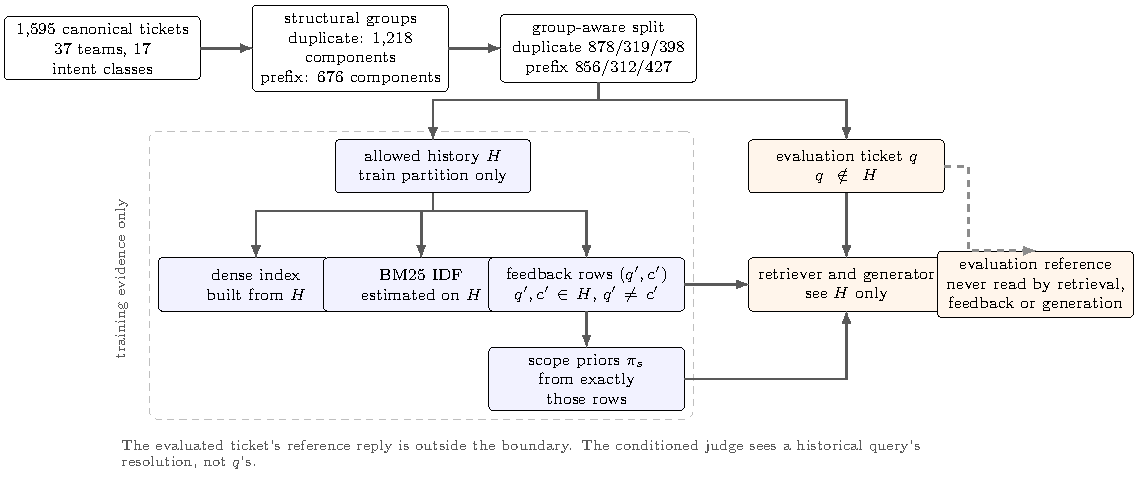
\includegraphics[width=\textwidth]{revision_ieee_access/03_manuscript/figures/fig1_regime.pdf}
\caption{Data regime and allowed history. The retriever, BM25 statistics, feedback
rows and scope priors see only the training partition $H$; the evaluation ticket's
reference reply stays outside the boundary. The conditioned judge uses a historical
query's resolution, not the evaluated ticket's reference.}
\label{fig:regime}
\end{figure*}

\subsection{Protocols and judges}
Feedback is produced twice, changing only what the judge sees. In the
\emph{conditioned} protocol the judge receives the training query, that query's
recorded resolution, and the candidate, and scores procedural equivalence on a
0--1 scale. Both the query and the candidate are historical tickets with known
resolutions, so the conditioned votes can be precomputed and used for a new query;
the judge never sees the new ticket's resolution. In the \emph{blind} protocol the
judge receives only the training query and the candidate, which is the setting
available for a new ticket at inference time. The contrast is therefore not between
an unrealizable upper bound and a deployable setting: it is a resolution-informed
judge on historical pairs versus a ticket-only judge.

Each protocol scores 878 training queries $\times$ 200 candidates $=$ 175,600
pairs at temperature 0 with a pinned model and run date. Each training query is
judged against 200 candidates, twice the evaluation pool, so that narrow scopes
retain enough documented evidence. The judge is the \texttt{gpt-5.6-luna} model at
temperature 0; the system prompt hash is \texttt{524098066b407de3}; the judging
cache dates are 12--13 September 2026. The same model is used for both protocols,
so the manipulation is what the judge sees, not which model judges.

The score distribution is zero-inflated and negative-heavy. On the allowed strict
rows, the conditioned judge assigns 62.9\,\% negative, 12.1\,\% positive and
25.0\,\% neutral scores; the blind judge assigns 57.3\,\%, 7.8\,\% and 34.9\,\%.
The full judged set contains 58.7\,\% and 48.3\,\% exact zeros. This asymmetry is a
property of the evidence, not of the lift formula, and it drives the saturation
analysis in Section~\ref{sec:repair}.

\subsection{Generation regime and provenance}
All primary runs share one generation regime: the \texttt{gpt-5.6-luna} model at
temperature 0. The system prompt hash is \texttt{524098066b407de3}; the regime
identifier is \texttt{51fd9f4b37e900bb}; and the response cache is warm. The
history-only panels were generated on 12 November 2026. Baseline answers are identical across sources of the
same panel; the freeze record in the repository verifies this ticket by ticket. The
cross-generator experiment in the earlier evaluation used a different model and is
not pooled with this study; the claims are within one regime. Because
hosted models can drift, all comparisons are within-regime and the artifacts record
the exact model, prompt and dates.

\subsection{Statistical protocol}
The estimand is the mean paired difference in cosine between the feedback and
baseline replies on the same tickets. We report a ticket-level paired bootstrap
interval for the mean and for the median, because the outcome is zero-inflated:
under conditioned feedback, 55.0\,\% of strict-panel and 22.6\,\% of familiar-panel
tickets have an unchanged answer. The median is exactly zero in most cells, so a
rank test has little power even when the mean interval excludes zero; we report the
Wilcoxon test as a secondary statistic and state which statistic each claim uses.
All intervals resample tickets as clusters. Paired tests are two-sided.

We fix three families before adjustment: conditioned and blind across
panels; reply similarity; and the direct conditioned-minus-blind contrast. Holm
correction is applied within each family. Exploratory analyses (scope grid, formula
ordering, expected-value selection, negative results) are labelled as such and are
not used for confirmation. The minimum detectable effect (MDE) at 80\,\% power is
reported for each primary cell; it is a sensitivity floor, not an equivalence
boundary. An earlier version of this evaluation used the eval split, so the
the analyses in this article are not prospectively preregistered. We state this explicitly
rather than claiming a registration that does not exist. The analysis protocol and
the frozen artifact hashes are dated and archived.

\subsection{Data availability and ethics}
The enterprise tickets are confidential and anonymized and cannot be released.
Organizational approval was obtained for research use. The code, judge prompts,
frozen scores, run manifests, aggregate tables and figure generators are released in
the project repository; the ticket text, feedback pairs and generated answers remain
closed because they contain confidential enterprise text. The repository includes a
license file: code is released under MIT and documentation and aggregate tables
under CC BY 4.0. The expert study used anonymized tickets, stored ratings without
ticket text in any external service, and reports only aggregates. Section~\ref{sec:repro}
states exactly what a third party can rerun.
